\documentclass[a4paper,11pt]{article}
\usepackage[margin=1.5cm]{geometry}

\usepackage{graphicx}
\usepackage{xcolor}
\usepackage{multirow}
\usepackage{tabularx}

\makeatletter
\newcommand{\useicon}[1]{\raisebox{-3pt}{\includegraphics[height=\dimexpr\f@size pt\relax]{./icons/#1.png}}}
\makeatother

\setlength{\tabcolsep}{3pt}
\setlength{\itemsep}{0pt}
\setlength{\parindent}{0pt}

\begin{document}
\begin{minipage}{0.2\textwidth}
	\centering
	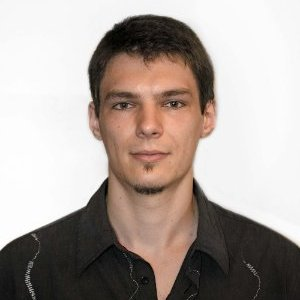
\includegraphics[width=2.5cm]{./gb.jpg}
\end{minipage}%
\begin{minipage}{0.4\textwidth}
	\fcolorbox{black}{blue!25}{\begin{tabular}{r c l}
		\multicolumn{3}{c}{Guillaume BONO} \\
		\hline
		born on &: &November 22\textsuperscript{nd}, 1992 \\
			 in &: &Bron, France
	\end{tabular}}
\end{minipage}%
\begin{minipage}{0.4\textwidth}
	\colorbox{yellow!35}{\begin{tabular}{r c l}
		\useicon{home} &:
			&22 rue Th{\'e}nard \\
		  & &69008, Lyon, France \\
		\useicon{phone} &:
			&+33 6 85 07 97 05 \\
		\useicon{mail} &:
			&\texttt{guillaume.bono@insa-lyon.fr}
	\end{tabular}}
\end{minipage}

\vspace{11pt}
\fcolorbox{black}{black!20}{\parbox{\textwidth}{\large\bf\centering Application to PhD degree}}

\section*{\useicon{research} Research activities}

\subsection*{Thesis}
\centering
\colorbox{orange!20}{\begin{tabular}{r c l}
	Title &: &Deep Multi-Agent Reinforcement Learning \\
	& &for Dynamic and Stochastic Vehicle Routing Problems \\
	Organization &: &INSA Lyon, INRIA, CITI \\
	Team &: &CHROMA \\
	Fundings &: &INSA/Volvo chair (3y) $+$ ATER (1y) \\
	Director &: &Olivier Simonin {\footnotesize (INSA Lyon, INRIA, CITI)} \\
	Academic supervisors &: &Jilles Dibangoye {\footnotesize (INSA Lyon, INRIA, CITI)} \\
	& &La{\"e}titia Matignon {\footnotesize (Universit{\'e} Lyon 1, LIRIS, CNRS)} \\
	Industrial supervisor &: &Florian Pereyron {\footnotesize (Volvo group)}
\end{tabular}}
\flushleft

\subsection*{Publications}
\resizebox{\textwidth}{!}{\begin{tabular}{c|r c l r c l}
	\multirow{3}{*}{\rotatebox{90}{\scriptsize Journal}}
	&Title      &: &Solving Multi-Agent Routing Problems using Deep Attention Mechanisms \\
	&Journal    &: &Transactions on Intelligent Transportation Systems \\
	&Publisher  &: &IEEE              &Date &: &July, 2020 \\
	\hline
	\multirow{10}{*}{\rotatebox{90}{\scriptsize Conferences}}
	&Title      &: &Cooperative Multi-agent Policy Gradient \\
	&Conference &: &European Conference on Machine Learning (ECML) \\
	&Location   &: &Dublin, Ireland   &Date &: &September, 2018 \\
	\cline{2-7}
	&Title      &: &Classification des probl{\`e}mes stochastiques et dynamiques \\
	& & &de collectes et de livraisons par des v{\'e}hicules intelligents \\
	&Conference &: &Journ{\'e}es Francophones sur la Planification, la Decision et l'Apprentissage (JFPDA) \\
	&Location   &: &Caen, France      &Date &: &July, 2017 \\
	\cline{2-7}
	&Title      &: &Sur le Gradient de la Politique pour les Syst{\`e}mes Multi-agents Coop{\'e}ratifs \\
	&Conference &: &Journ{\'e}es Francophones sur la Planification, la Decision et l'Apprentissage (JFPDA) \\
	&Location   &: &Nancy, France     &Date &: &July, 2018 \\
	\hline
	\multirow{4}{*}{\rotatebox{90}{\scriptsize Workshop}}
	&Title      &: &Simulation of Stochastic Vehicle Routing Problems in Urban Environment \\
	&Workshop   &: &Prediction and Generative Modeling in Reinforcement Learning (PGMRL) \\
	&at         &: &Federated AI Meeting (AAMAS, ICML, and IJCAI) \\
	&Location   &: &Stockholm, Sweden &Date &: &July, 2018 \\
\end{tabular}}

\subsection*{Summer schools}
\centering
\begin{tabular}{r c l r c l}
	Title &: &1\textsuperscript{st} Summer School on Cognitive Robotics \\
	Organizers &: &MERS group, MIT CSAIL \\
	Location &: &Cambridge, MA, USA &Date &: &June, 2017 \\
	\hline
	Title &: &1\textsuperscript{er} Institut d'Automne en Intelligence Artificielle \\
	Organizers &: &GdR IA \\
	Location &: &Lyon, France       &Date &: &October, 2017 \\
	\hline
	Title &: &3\textsuperscript{{\`e}me} Institut d'Automne en Intelligence Artificielle \\
	Organizers &: &GdR IA \\
	Location &: &Lyon, France       &Date &: &October, 2019 \\
\end{tabular}
\flushleft

\section*{\useicon{teach} Teaching activities}
\begin{tabularx}{\textwidth}{l X c c c c}
	\itshape Name &\itshape Description &\multicolumn{2}{c}{\itshape Class} &\itshape Hours &\itshape Year \\
	\hline
	PIT  &Initiation to command line (bash) and programming (C, python)
		&3TC &(UGRD) &24h        &2018-19 \\
		&&&          &$\times 2$ &2019-20 \\
	PPC  &Practical sessions and projects on parallel programming (python)
		&3TC &(UGRD) &22h &2019-20 \\
	WEB  &Tutorials and projects on dynamic web development
		&3TC &(UGRD) &34h &2019-20 \\
	CRO  &Practical sessions on basics of programming in C
		&3TC &(UGRD) &18h &2019-20 \\
	MAC  &Tutorials and practical sessions on Medium Access Control
		&3TC &(UGRD) &16h &2019-20 \\
	IP   &Practical sessions on Internet Protocol
		&3TC &(UGRD) &10h &2019-20 \\
	DBM2 &Lectures and tutorials on Data Mining (in English)
		&IST &(UGRD) &20h &2019-20 \\
	SMR  &Practical sessions and projects with robots (ROS, android)
		&5TC &(GRAD) &12h        &2018-19 \\
		&&&          &$\times 2$ &2019-20 \\
	CSAD &Tutorials and practical sessions on Network Science
		&5TC &(GRAD) &6h  &2019-20 \\
\end{tabularx}
\flushright
{\itshape All teaching activities were conducted in the Telecom department of INSA Lyon.}
\flushleft

\section*{\useicon{edu} Education}
\begin{tabularx}{\textwidth}{r >{\footnotesize}l c X r}
	Georgia Tech      &(Atlanta, GA, USA)       &: &\bf Master of Computer Science &December, 2015 -- \\
	&&&\footnotesize computer perceptions and robotics &-- May, 2015 \\
	Sup{\'e}lec $\times$ &(Metz, France)           &: &\bf Engineering Degree &August, 2014 --\\
	GATech Lorraine&&&\footnotesize interactive systems and robotics, Machine Learning &-- July, 2015 \\
	 &(Gif-sur-Yvette, France) &: &\footnotesize algorithms, software dev., electronics, control,
	 &September, 2012 --\\
	&&&\footnotesize economy, management, $\dots$ &-- August, 2014 \\
	La Martini{\`e}re &(Lyon, France)           &: &Preparatory classes &September, 2010 --\\
	Monplaisir &&&\footnotesize mathematics, physics and engineering &-- August, 2012 \\
	La Martini{\`e}re &(Lyon, France)           &: &\bf High-school diploma &September, 2006 --\\
	Monplaisir &&&&-- August, 2010 \\
\end{tabularx}

\section*{\useicon{work} Professional experience}
\begin{tabularx}{\textwidth}{r c X r}
	Awabot &: &Internship and Research Engineer \\
		&&integrating gestures recognition into a home companion robot    &August, 2015 -- \\
		&&implementing a DNN using \emph{Caffe} on a \emph{nVidia Tegra K1} &-- December, 2015 \\
\end{tabularx}

\section*{\useicon{perso} Personal experience}
\begin{tabularx}{\textwidth}{r c X r}
	Sono Sup{\'e}lec &:
		&Venue organization and logistics, events animation, light shows, &October, 2012 -- \\
		&&live audio engineer, technical troubleshooting &-- August, 2014 \\
\end{tabularx}

\vspace{11pt}
\begin{minipage}[t]{0.3\textwidth}
	\section*{\useicon{lang} Languages}
	\begin{tabular}{r l r}
		\useicon{fr-flag} &French  &C2 \\
		\useicon{uk-flag} &English &C1 \\
		\useicon{de-flag} &German  &B2-C1 \\
		\useicon{cn-flag} &Chinese &A1 \\
	\end{tabular}
\end{minipage}\hfill
\begin{minipage}[t]{0.34\textwidth}
	\section*{\useicon{comp} Computer skills}
	\centering
	C, C++, python, java \\
	typescript, javascript, sql \\
	stdlib, boost, openCV, openNI \\
	ROS, CUDA \\
	pytorch, numpy, scipy, pandas \\
	android, angular, express, mongodb \\
	git, subversion \\
	LaTeX, Office
\end{minipage}\hfill
\begin{minipage}[t]{0.3\textwidth}
	\section*{\useicon{games} Hobbies}
	\flushright
	Video-games, e-Sport \\
	Computer Hardware, Robots \\
	Music, Guitar \\
	Sound systems, Audio engineer \\
	Board-games, RPG \\
	Books and films: Fantasy, SF 
\end{minipage}
\end{document}
